%%%%%%%%%%%%%%%%%%%%%%%%
%
% $Autor: Wings $
% $Project:  $
% $Filename: MosfetRF520.tex $
% $Short description: In diesem Abschnitt wird der Aktor "Entwicklerboard mit MOSFET IRF520" genauer beschrieben. Es werden der allgemeine Aufbau und die Funktionsweise eines MOSFETs erläutert. Zudem wird das verwendete Entwicklerboard detailliert vorgestellt. Abschließend erfolgt eine Erklärung der PWM-Signale sowie eine Darstellung passender Codebeispiele. $
%
%%%%%%%%%%%%

\chapter{Entwicklerboard mit MOSFET IRF520}
\label{sec:mosfet}

\section{MOSFET-Treibermodul (IRF520)}

Das IRF520-Modul ist ein auf einem N-Kanal-Leistungs-MOSFET basierendes Treibermodul, das sich für einfache Schalt- und PWM-Anwendungen mit Mikrocontrollern eignet. Es wird häufig zur Ansteuerung von Gleichstrommotoren, LEDs oder anderen Lasten im Niederspannungsbereich verwendet. Im Gegensatz zu modernen Logikpegel-MOSFETs benötigt der IRF520 jedoch höhere Gate-Spannungen, um vollständig durchzuschalten, was seine Effizienz bei 3,3\,V-Logiksignalen einschränkt. Für 5\,V-Steuerung ist das Modul bedingt geeignet.\cite{OpenPlatform.cc.2020}

Das Modul enthält neben dem eigentlichen MOSFET auch eine Anschlussklemme für die zu schaltende Last, einen Gate-Widerstand und eine Freilaufdiode (z.\,B.\ 1N4007), was es besonders für Einsteiger geeignet macht. Die Schaltung ist so ausgelegt, dass über ein PWM-Signal direkt der Gate-Anschluss angesteuert werden kann.

Eigenschaften des IRF520 sind eine maximale \textit{Drain-Source-Spannung} von \textbf{100\,V} und ein maximaler Strom von \textbf{9,2\,A}. Der typische Einschaltwiderstand beträgt etwa \textbf{0{,}27\,$\Omega$} bei $V_{\text{GS}} = 10\,\text{V}$, was bei höheren Lasten zu relevanten Verlustleistungen führen kann. Für Anwendungen mit hohen Strömen oder geringem Spannungsabfall ist daher ein leistungsfähigerer MOSFET mit Logic-Level-Eigenschaften zu bevorzugen.

Das Modul eignet sich gut für Experimente und Lasterprobungen im unteren Leistungsbereich. Bei einer PWM-Ansteuerung sollte beachtet werden, dass der IRF520 nicht als Logic-Level-MOSFET konzipiert ist.

\bigskip
\begin{center}
    
\includegraphics[width=4cm]{Mosfet/MosfetIRF520}
    \captionof{figure}{MOSFET-Treibermodul mit IRF520}
    \label{fig:mosfetirf520}
\end{center}



\section{Allgemein}

Ein MOSFET (Metal-Oxide-Semiconductor Field-Effect Transistor) ist ein spannungsgesteuerter Halbleiterbaustein, der in der Elektronik sowohl zum Schalten als auch zur Verstärkung von elektrischen Signalen eingesetzt wird. Er zählt zur Familie der Feldeffekttransistoren (FET) und zeichnet sich durch seine hohe Eingangsimpedanz sowie geringe Leistungsverluste aus. \cite{Hering.2021}

\subsection{Aufbau und Funktionsweise}

Wie in Abbildung \ref{fig:AufbauMOSFETs} dargestellt verfügt ein MOSFET über drei Anschlüsse:
\begin{itemize}
	\item \textbf{Gate (G)}: Steuerelektrode
	\item \textbf{Drain (D)}: Stromsenke
	\item \textbf{Source (S)}: Stromquelle
\end{itemize}


\begin{center}
  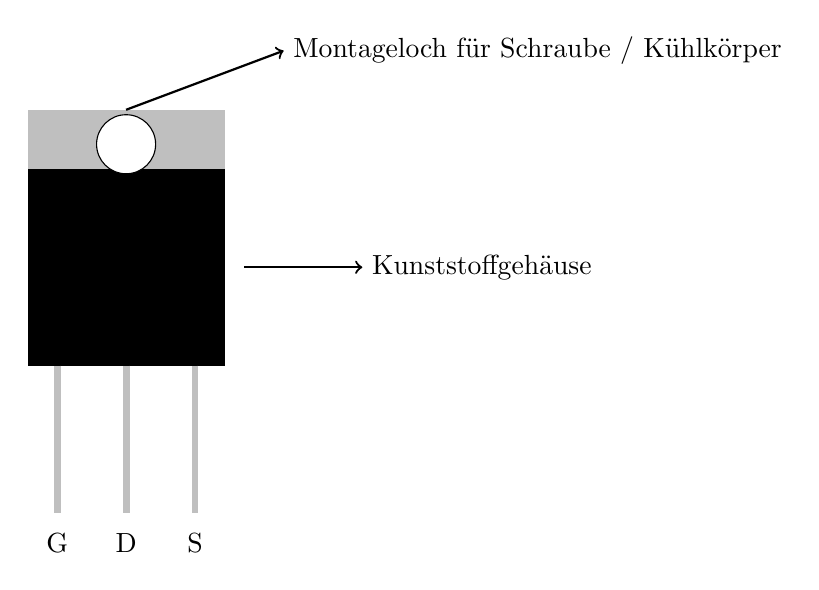
\begin{tikzpicture}[scale=2.5] 
    
    % Gehäuse
    \fill[black] (-0.5,0) rectangle (0.5,1);
    
    % Metalllasche oben
    \fill[gray!50] (-0.5,1) rectangle (0.5,1.3);
    \draw[fill=white] (0,1.125) circle (0.15); % Loch
    
    % Pins
    \foreach \x in {-0.35, 0, 0.35} {
        \draw[gray!50, line width=2.5pt] (\x,0) -- (\x,-0.75);
    }
    
    % Beschriftung der Pins
    \node[font=\normalsize] at (-0.35,-0.9) {G};
    \node[font=\normalsize] at (0,-0.9) {D};
    \node[font=\normalsize] at (0.35,-0.9) {S};
    
    % Beschriftung Gehäuse
    \draw[->, thick] (0.6,0.5) -- (1.2,0.5);
    \node[anchor=west, font=\normalsize] at (1.2,0.5) {Kunststoffgehäuse};
    
    % Beschriftung Montageloch
    \draw[->, thick] (0,1.3) -- (0.8,1.6);
    \node[anchor=west, font=\normalsize] at (0.8,1.6) {Montageloch für Schraube / Kühlkörper};
    
  \end{tikzpicture}
  \captionof{figure}{Aufbau eines MOSFETs}
\label{fig:AufbauMOSFETs}
\end{center}



Die Steuerung des Stromflusses zwischen Source und Drain erfolgt durch Anlegen einer Spannung am Gate. Eine isolierende Oxidschicht trennt das Gate vom Halbleitermaterial, wodurch nahezu kein Strom in das Gate fließt. Je nach angelegter Gate-Source-Spannung bildet sich ein leitfähiger Kanal aus, der den Stromfluss ermöglicht oder unterbindet.

\subsection{Typen von MOSFETs}

MOSFETs lassen sich in folgende Haupttypen unterteilen:

\begin{itemize}
	\label{sec:NKanalMOSFETs}
	\item \textbf{N-Kanal-MOSFETs}: Leiten Strom, wenn eine positive Spannung am Gate anliegt.
	\item \textbf{P-Kanal-MOSFETs}: Leiten Strom bei negativer Gate-Spannung.
\end{itemize}

Zudem existieren zwei Betriebsmodi:
\begin{itemize}
	\item \textbf{Anreicherungstyp (Enhancement Mode)}: Standardmäßig nichtleitend; leitet erst bei Anlegen einer geeigneten Gate-Spannung.
	\item \textbf{Verarmungstyp (Depletion Mode)}: Standardmäßig leitend; der Stromfluss kann durch Gate-Spannung reduziert oder unterbrochen werden.
\end{itemize}

Der N-Kanal-Anreicherungstyp ist der am häufigsten verwendete MOSFET-Typ in der Praxis.


\subsection{PWM-Steuerung}

Die PWM-Steuerung (Pulsweitenmodulation) ist ein Verfahren zur Erzeugung einer variablen mittleren Ausgangsspannung bei konstanter Versorgungsspannung. Die PWM-Steuerung basiert auf einem digitalen Rechtecksignal mit konstanter Frequenz und variabler Einschaltzeit. Das Verhältnis der Einschaltzeit zur Gesamtzykluszeit wird als Tastverhältnis bezeichnet. Die PWM-Steuerung erlaubt es, den MOSFET IRF520 in sehr kurzen Zeitabständen ein- und auszuschalten. Durch die Trägheit der Fahrzeuge ergibt sich für die Motoren eine geglättete mittlere Spannung, die proportional zum Tastverhältnis des PWM-Signals ist. Die PWM-Steuerung in Kombination mit dem MOSFET IRF520 ermöglicht somit eine verlustarme, feinfühlige und energieeffiziente Regelung. Die PWM-Steuerung ist eine bewährte Methode zur Leistungsregelung in der Antriebstechnik und kommt auch in industriellen Anwendungen und Konsumgütern zum Einsatz. \cite{Gehrke.2022}



\section{Entwicklerboard mit MOSFET IRF520}

\textbf{Verwendeter Aktor: IRF520 N-Kanal MOSFET}

Der in diesem Projekt eingesetzte Aktor ist ein N-Kanal-Leistungs-MOSFET vom Typ IRF520 und in Abbildung \ref{fig:MOSFETIRF520} dargestellt. Dieser dient als elektronischer Schalter zur Ansteuerung von Gleichstromverbrauchern. Er eignet sich besonders für Anwendungen, bei denen mit Hilfe von PWM-Signalen Lasten geschaltet oder geregelt werden sollen. \cite{OpenPlatform.cc.2020}

\begin{center}
\begin{tikzpicture}
    
    \tikzstyle{every node}=[font=\normalsize]
    \draw [ fill={rgb,255:red,255; green,15; blue,8} ] (9,22.25) rectangle (21.75,14.75);
    \draw [ color={rgb,255:red,140; green,140; blue,140} , fill={rgb,255:red,214; green,214; blue,214}, line width=1pt ] (21,18.5) circle (0.5cm);
    \draw [ fill={rgb,255:red,22; green,107; blue,218} ] (16.5,21.75) rectangle (19.5,20.25);
    \draw [ color={rgb,255:red,140; green,140; blue,140} , fill={rgb,255:red,214; green,214; blue,214}, line width=1pt ] (10,18.5) circle (0.5cm);
    \draw [ fill={rgb,255:red,22; green,107; blue,218} ] (11.25,21.75) rectangle (14.25,20.25);
    \draw [ fill={rgb,255:red,140; green,140; blue,140} ] (12,21) circle (0.5cm);
    \draw [ fill={rgb,255:red,140; green,140; blue,140} ] (13.5,21) circle (0.5cm);
    \draw [ fill={rgb,255:red,140; green,140; blue,140} ] (17.25,21) circle (0.5cm);
    \draw [ fill={rgb,255:red,140; green,140; blue,140} ] (18.75,21) circle (0.5cm);
    \draw [ fill={rgb,255:red,0; green,0; blue,0} ] (11.5,17) rectangle (14,16);
    \draw [ fill={rgb,255:red,140; green,140; blue,140} ] (17.5,15.25) rectangle (17.75,13.5);
    \node [font=\LARGE] at (18.25,13.75) {};
    \draw [ fill={rgb,255:red,140; green,140; blue,140} ] (18.25,15.25) rectangle (18.5,13.5);
    \node [font=\LARGE] at (18.75,13.25) {};
    \node [font=\LARGE] at (18.75,13.25) {};
    \node [font=\LARGE] at (18.75,13.25) {};
    \node [font=\LARGE] at (18.75,13.25) {};
    \node [font=\LARGE] at (19.25,12.75) {};
    \node [font=\LARGE] at (19,12.75) {};
    \draw [ fill={rgb,255:red,140; green,140; blue,140} ] (19,15.25) rectangle (19.25,13.5);
    \draw [ fill={rgb,255:red,120; green,120; blue,120} ] (11.5,17) rectangle (14,16.75);
    \node [font=\large, rotate around={90:(0,0)}] at (21,16.5) {Mos Module};
    \node [font=\large] at (17,15) {SIG};
    \node [font=\large] at (18.25,15.5) {VCC};
    \node [font=\large] at (20,15) {GND};
    \node [font=\large] at (11.75,19.75) {V+};
    \node [font=\large] at (13.5,19.75) {V-};
    \node [font=\large] at (17.25,19.75) {VIN};
    \node [font=\large] at (18.75,19.75) {GND};
    \node [font=\large] at (12.75,17.5) {MOSFET IRF520};
    \draw [ color={rgb,255:red,99; green,99; blue,99}, , line width=2pt](12,21.5) to[short] (12,20.5);
    \draw [ color={rgb,255:red,99; green,99; blue,99}, , line width=2pt](13.5,21.5) to[short] (13.5,20.5);
    \draw [ color={rgb,255:red,99; green,99; blue,99}, , line width=2pt](17.25,21.5) to[short] (17.25,20.5);
    \draw [ color={rgb,255:red,99; green,99; blue,99}, , line width=2pt](18.75,21.5) to[short] (18.75,20.5);
    \node [font=\LARGE] at (19.75,10.25) {};
    \node [font=\LARGE] at (19.75,10.25) {};
    \node [font=\LARGE] at (23.25,10.5) {};
    \node [font=\LARGE] at (23.25,10.5) {};
    \node [font=\LARGE] at (23.75,10) {};
    \node [font=\LARGE] at (18.75,13.25) {};
    \draw [line width=1pt, short] (10.5,23) -- (11.5,21.5);
    \node [font=\LARGE] at (10.5,23.5) {Schraubklemmen};
    \draw [line width=1pt, short] (19.25,13.5) -- (20.25,12.5);
    \node [font=\LARGE] at (20.75,12) {Stiftleiste};
    
  \end{tikzpicture}
  \captionof{figure}{MOSFET IRF520}
  \label{fig:MOSFETIRF520}
\end{center}

\bigskip

\begin{itemize}
	\item \textbf{Typ:} IRF520 N-Kanal MOSFET
	\item \textbf{Modulspannung (Steuerspannung):} 3{,}3\,V 
	\item \textbf{Maximale Lastspannung (Drain-Source):} 24\,V
	\item \textbf{Maximaler Laststrom:} bis ca. 5\,A
\end{itemize}
 \newpage

Das Entwicklerboard mit MOSFET IRF520 wird in diesem Projekt eingesetzt, um die Spannung auf den Schienen einer Carrera-Bahn zu regeln.\cite{OpenPlatform.cc.2020} Bei PWM-Durchschaltung gibt das Entwicklerboard mit MOSFET IRF520 die vom Netzteil anliegende Spannung von 18\,V an die Carrerabahn weiter. Der verbaute MOSFET IRF520 wird dabei durch ein PWM-Signal des Arduino Nano 33 BLE Sense Lite angesteuert. Für die Signalübertragung wurde der PWM-fähige Pin D9 verwendet; alternativ stehen auch die Pins D2, D3, D5, D6 sowie D10 bis D12 zur Verfügung.\cite{Arduino.2025b}
Die einzelnen Komponenten des Schaltungsaufbaus sind in Abbildung~\ref{fig:MOSFET_PWM_Schaltung} dargestellt und lassen sich wie folgt beschreiben:

\begin{itemize}
	\item \textbf{SIG} $\rightarrow$ \textbf{D9} am Arduino Nano 33 BLE Sense Lite \\
	(Steuersignal über PWM zur Geschwindigkeitsregelung vom Arduino zum Modul)\\
	\textit{Verbindung: Steckbrücken-Kabel}
	
	\item \textbf{VCC} $\rightarrow$ \textbf{3V3} am Arduino \\
	(Versorgung der Logik auf dem Modul und der Status-LED)\\
	\textit{Verbindung: Steckbrücken-Kabel}
	
	\item \textbf{GND} (Pinleiste) $\rightarrow$ \textbf{GND} am Arduino \\
	(gemeinsame Masse zwischen Arduino und Modul)\\
	\textit{Verbindung: Steckbrücken-Kabel}
	
	\item \textbf{GND} (Schraubklemme) $\rightarrow$ \textbf{GND} vom Netzteil \\
	(gemeinsame Masse für die Lastversorgung)\\
	\textit{Verbindung: Litze, 0{,}5--1{,}0\,mm\textsuperscript{2}}
	
	\item \textbf{VIN} (Schraubklemme) $\rightarrow$ \textbf{+18\,V} von der Carrerabahn \\
	(Versorgungsspannung von Netzteil über Carrerabahn)\\
	\textit{Verbindung: Litze, 0{,}5--1{,}0\,mm\textsuperscript{2}}
	
	\item \textbf{V$-$} (Schraubklemme) $\rightarrow$ \textbf{Minuspol der Carrera-Bahn} \\
	(geschalteter Pfad zum Verbraucher, wird über den MOSFET mit GND verbunden)\\
	\textit{Verbindung: Litze, 0{,}5--1{,}0\,mm\textsuperscript{2}}
	
\end{itemize}

\begin{center}
\begin{circuitikz}
    \tikzstyle{every node}=[font=\LARGE]
    \draw [ fill={rgb,255:red,247; green,159; blue,8} ] (9,22.25) rectangle (21.75,14.75);
    \draw [ color={rgb,255:red,140; green,140; blue,140} , fill={rgb,255:red,214; green,214; blue,214}, line width=1pt ] (21,18.5) circle (0.5cm);
    \draw [ fill={rgb,255:red,22; green,107; blue,218} ] (16.5,21.75) rectangle (19.5,20.25);
    \draw [ color={rgb,255:red,140; green,140; blue,140} , fill={rgb,255:red,214; green,214; blue,214}, line width=1pt ] (10,18.5) circle (0.5cm);
    \draw [ fill={rgb,255:red,22; green,107; blue,218} ] (11.25,21.75) rectangle (14.25,20.25);
    \draw [ fill={rgb,255:red,140; green,140; blue,140} ] (12,21) circle (0.5cm);
    \draw [ fill={rgb,255:red,140; green,140; blue,140} ] (13.5,21) circle (0.5cm);
    \draw [ fill={rgb,255:red,140; green,140; blue,140} ] (17.25,21) circle (0.5cm);
    \draw [ fill={rgb,255:red,140; green,140; blue,140} ] (18.75,21) circle (0.5cm);
    \draw [ fill={rgb,255:red,0; green,0; blue,0} ] (11.5,17) rectangle (14,16);
    \draw [ fill={rgb,255:red,140; green,140; blue,140} ] (17,15.25) rectangle (17.5,13.5);
    \node [font=\LARGE] at (18.25,13.75) {};
    \draw [ fill={rgb,255:red,140; green,140; blue,140} ] (18,15.25) rectangle (18.5,13.5);
    \node [font=\LARGE] at (18.75,13.25) {};
    \node [font=\LARGE] at (18.75,13.25) {};
    \node [font=\LARGE] at (18.75,13.25) {};
    \node [font=\LARGE] at (18.75,13.25) {};
    \node [font=\LARGE] at (19.25,12.75) {};
    \node [font=\LARGE] at (19,12.75) {};
    \draw [ fill={rgb,255:red,140; green,140; blue,140} ] (19,15.25) rectangle (19.5,13.5);
    \draw [ fill={rgb,255:red,120; green,120; blue,120} ] (11.5,17) rectangle (14,16.75);
    \node [font=\large, rotate around={90:(0,0)}] at (21,16.5) {Mos Module};
    \node [font=\large] at (16.5,15) {SIG};
    \node [font=\large] at (18.25,15.5) {VCC};
    \node [font=\large] at (20.25,15) {GND};
    \node [font=\large] at (11.75,19.75) {V+};
    \node [font=\large] at (13.5,19.75) {V-};
    \node [font=\large] at (17.25,19.75) {VIN};
    \node [font=\large] at (18.75,19.75) {GND};
    \node [font=\large] at (12.75,17.5) {MOSFET IRF520};
    \draw [ color={rgb,255:red,99; green,99; blue,99}, , line width=2pt](12,21.5) to[short] (12,20.5);
    \draw [ color={rgb,255:red,99; green,99; blue,99}, , line width=2pt](13.5,21.5) to[short] (13.5,20.5);
    \draw [ color={rgb,255:red,99; green,99; blue,99}, , line width=2pt](17.25,21.5) to[short] (17.25,20.5);
    \draw [ color={rgb,255:red,99; green,99; blue,99}, , line width=2pt](18.75,21.5) to[short] (18.75,20.5);
    \draw [ color={rgb,255:red,255; green,255; blue,255} , fill={rgb,255:red,24; green,112; blue,119}] (18.5,12) rectangle (22.75,0.5);
    \node [font=\LARGE] at (19.75,10.25) {};
    \node [font=\LARGE] at (19.75,10.25) {};
    \draw [ fill={rgb,255:red,140; green,140; blue,140} ] (19,10.25) circle (0.25cm);
    \draw [ fill={rgb,255:red,230; green,229; blue,229} ] (19,11.5) circle (0.25cm);
    \draw [ fill={rgb,255:red,230; green,229; blue,229} ] (22.25,11.5) circle (0.25cm);
    \draw [ fill={rgb,255:red,230; green,229; blue,229} ] (22.25,1) circle (0.25cm);
    \node [font=\LARGE] at (23.25,10.5) {};
    \node [font=\LARGE] at (23.25,10.5) {};
    \node [font=\LARGE] at (23.75,10) {};
    \draw [ fill={rgb,255:red,230; green,229; blue,229} ] (19,1) circle (0.25cm);
    \draw [ color={rgb,255:red,250; green,0; blue,0}, line width=1pt, short] (19,10) -- (19,9.25);
    \draw [ color={rgb,255:red,255; green,0; blue,0}, line width=1pt, short] (19,9.25) -- (18.25,9.25);
    \draw [ color={rgb,255:red,255; green,255; blue,255} , fill={rgb,255:red,255; green,0; blue,0}] (15.75,9.5) rectangle (18.25,9);
    \node [font=\large, color={rgb,255:red,232; green,232; blue,232}] at (16.5,9.25) {+3V3};
    \draw [ color={rgb,255:red,255; green,255; blue,255} , fill={rgb,255:red,230; green,230; blue,230}] (17.25,9.5) rectangle (18.25,9);
    \node [font=\large, color={rgb,255:red,255; green,0; blue,0}] at (17.75,9.25) {OUT};
    \draw [ color={rgb,255:red,0; green,132; blue,255}, , line width=2pt](19,10.25) to[short] (18.25,10.25);
    \draw [ color={rgb,255:red,0; green,132; blue,255}, , line width=2pt](18.25,10.25) to[short] (18.25,13.75);
    \draw [ fill={rgb,255:red,0; green,0; blue,0} ] (18,14) rectangle (18.5,13.5);
    \draw [ fill={rgb,255:red,140; green,140; blue,140} ] (19,2.5) circle (0.25cm);
    \draw [line width=1pt, short] (19,2.25) -- (19,1.75);
    \draw [line width=1pt, short] (19,1.75) -- (18.25,1.75);
    \draw [ color={rgb,255:red,232; green,232; blue,232} , fill={rgb,255:red,0; green,0; blue,0}, line width=1pt ] (16.75,2) rectangle  node {\large GND} (18.25,1.5);
    \draw [line width=2pt, short] (19,2.5) -- (15.5,2.5);
    \draw [line width=2pt, short] (15.5,2.5) -- (15.5,12.5);
    \draw [line width=2pt, short] (15.5,12.5) -- (19.25,12.5);
    \draw [line width=2pt, short] (19.25,12.5) -- (19.25,13.5);
    \node [font=\LARGE] at (18.75,13.25) {};
    \draw [ fill={rgb,255:red,0; green,0; blue,0} ] (19,14) rectangle (19.5,13.5);
    \draw [ fill={rgb,255:red,140; green,140; blue,140} ] (22.25,8.5) circle (0.25cm);
    \draw [ color={rgb,255:red,255; green,115; blue,0}, line width=1pt, short] (22.25,8.25) -- (22.25,7.5);
    \draw [ color={rgb,255:red,255; green,136; blue,0}, line width=1pt, short] (22.25,7.5) -- (23,7.5);
    \draw [ color={rgb,255:red,255; green,255; blue,255} , fill={rgb,255:red,255; green,162; blue,0}, line width=1pt ] (23,7.75) rectangle  node {\large D9} (24.5,7.25);
    \draw [ color={rgb,255:red,0; green,255; blue,0}, line width=2pt, short] (22.25,8.5) -- (23.25,8.5);
    \draw [ color={rgb,255:red,0; green,255; blue,0}, line width=2pt, short] (23.25,8.5) -- (23.25,13);
    \draw [ color={rgb,255:red,0; green,255; blue,0}, line width=2pt, short] (23.25,13) -- (17.25,13);
    \draw [ color={rgb,255:red,0; green,255; blue,0}, line width=2pt, short] (17.25,13) -- (17.25,13.5);
    \draw [ fill={rgb,255:red,0; green,0; blue,0} ] (17,14) rectangle (17.5,13.5);
    \draw [ fill={rgb,255:red,59; green,59; blue,59} ] (5.25,31.25) rectangle (26.25,27);
    \draw [ fill={rgb,255:red,33; green,33; blue,33} ] (9.75,28) rectangle (21.5,27);
    \draw [ fill={rgb,255:red,86; green,82; blue,82} ] (14,27.5) circle (0.25cm);
    \node [font=\LARGE] at (14.75,27) {};
    \node [font=\LARGE] at (14.75,27) {};
    \draw [ fill={rgb,255:red,86; green,82; blue,82} ] (14.75,27.5) circle (0.25cm);
    \draw [ fill={rgb,255:red,86; green,82; blue,82} ] (16.75,27.5) circle (0.25cm);
    \draw [ fill={rgb,255:red,86; green,82; blue,82} ] (17.5,27.5) circle (0.25cm);
    \node [font=\LARGE, color={rgb,255:red,230; green,230; blue,230}] at (14,27.5) {+};
    \draw [ color={rgb,255:red,59; green,59; blue,59} , fill={rgb,255:red,179; green,0; blue,0}] (8.25,27) -- (9.25,27) -- (9.75,28) -- (8.75,28) -- cycle;
    \draw [ color={rgb,255:red,59; green,59; blue,59} , fill={rgb,255:red,235; green,235; blue,235}] (7.25,27) -- (8.25,27) -- (8.75,28) -- (7.75,28) -- cycle;
    \draw [ color={rgb,255:red,59; green,59; blue,59} , fill={rgb,255:red,179; green,0; blue,0}] (6.25,27) -- (7.25,27) -- (7.75,28) -- (6.75,28) -- cycle;
    \draw [ color={rgb,255:red,59; green,59; blue,59} , fill={rgb,255:red,235; green,235; blue,235}] (5.25,27) -- (6.25,27) -- (6.75,28) -- (5.75,28) -- cycle;
    \draw [ color={rgb,255:red,59; green,59; blue,59} , fill={rgb,255:red,235; green,235; blue,235}] (21.75,27) -- (22.75,27) -- (23.25,28) -- (22.25,28) -- cycle;
    \draw [ color={rgb,255:red,59; green,59; blue,59} , fill={rgb,255:red,179; green,0; blue,0}] (22.75,27) -- (23.75,27) -- (24.25,28) -- (23.25,28) -- cycle;
    \draw [ color={rgb,255:red,59; green,59; blue,59} , fill={rgb,255:red,235; green,235; blue,235}] (23.75,27) -- (24.75,27) -- (25.25,28) -- (24.25,28) -- cycle;
    \draw [ color={rgb,255:red,59; green,59; blue,59} , fill={rgb,255:red,179; green,0; blue,0}] (24.75,27) -- (25.75,27) -- (26.25,28) -- (25.25,28) -- cycle;
    \node [font=\LARGE, color={rgb,255:red,230; green,230; blue,230}] at (16.75,27.5) {+};
    \node [font=\LARGE, color={rgb,255:red,230; green,230; blue,230}] at (14.75,27.5) {-};
    \node [font=\LARGE, color={rgb,255:red,230; green,230; blue,230}] at (17.5,27.5) {-};
    \draw [ fill={rgb,255:red,28; green,28; blue,28} ] (5.25,31.25) rectangle (26.25,28.25);
    \draw [ fill={rgb,255:red,191; green,191; blue,191} ] (5,30.25) rectangle (26.25,30);
    \draw [ line width=2pt](14.75,27.25) to[short] (14.75,24.25);
    \draw [ fill={rgb,255:red,86; green,82; blue,82} ] (19,26.25) rectangle (21,23.25);
    \node [font=\LARGE, color={rgb,255:red,230; green,230; blue,230}] at (19.5,25.5) {+};
    \draw [ color={rgb,255:red,255; green,0; blue,0}, , line width=2pt](19.25,25.5) to[short] (14,25.5);
    \draw [ color={rgb,255:red,255; green,0; blue,0}, , line width=2pt](14,25.5) to[short] (14,27.25);
    \node [font=\LARGE, color={rgb,255:red,230; green,230; blue,230}] at (19.5,24.25) {-};
    \node [font=\LARGE] at (15.5,31.75) {Carrerabahn};
    \node [font=\LARGE] at (22.25,24.75) {Netzteil};
    \node [font=\LARGE] at (20.75,-0.25) {Arduino Nano 33 BLE Sense Lite};
    \node [font=\LARGE] at (6,19.25) {Entwicklerboard mit };
    \node [font=\LARGE] at (6.5,18.25) {MOSFET IRF520};
    \node [font=\LARGE] at (14.5,27) {};
    \draw [ fill={rgb,255:red,86; green,82; blue,82} ] (12.25,27.5) circle (0.25cm);
    \node [font=\LARGE] at (15,26.5) {};
    \draw [ fill={rgb,255:red,86; green,82; blue,82} ] (11.5,27.5) circle (0.25cm);
    \draw [ fill={rgb,255:red,86; green,82; blue,82} ] (10.75,27.5) circle (0.25cm);
    \draw [ fill={rgb,255:red,86; green,82; blue,82} ] (19.25,27.5) circle (0.25cm);
    \draw [ fill={rgb,255:red,86; green,82; blue,82} ] (20,27.5) circle (0.25cm);
    \draw [ fill={rgb,255:red,86; green,82; blue,82} ] (20.75,27.5) circle (0.25cm);
    \node [font=\LARGE, color={rgb,255:red,230; green,230; blue,230}] at (12.25,27.5) {-};
    \node [font=\LARGE, color={rgb,255:red,230; green,230; blue,230}] at (20,27.5) {-};
    \node [font=\LARGE, color={rgb,255:red,230; green,230; blue,230}] at (11.5,27.5) {+};
    \node [font=\LARGE, color={rgb,255:red,230; green,230; blue,230}] at (19.25,27.5) {+};
    \draw [ color={rgb,255:red,255; green,255; blue,255}, line width=1pt, dashed] (5.25,31) -- (26.25,31);
    \draw [ color={rgb,255:red,255; green,255; blue,255}, line width=1.5pt, short] (5.25,28.75) -- (26.25,28.75);
    \draw [ color={rgb,255:red,255; green,0; blue,0}, , line width=2pt](11.5,27.25) to[short] (11.5,22.75);
    \draw [ color={rgb,255:red,255; green,0; blue,0}, , line width=2pt](11.5,22.75) to[short] (17.25,22.75);
    \draw [ line width=2pt](12.25,27.25) to[short] (12.25,25);
    \draw [ line width=2pt](12.25,25) to[short] (13.5,25);
    \draw [ line width=2pt](13.5,25) to[short] (13.5,21.5);
    \draw [ line width=2pt](14.75,24.25) to[short] (19.25,24.25);
    \draw [ line width=2pt](19.25,13.25) to[short] (22.25,13.25);
    \draw [ line width=2pt](22.25,13.25) to[short] (22.25,22.75);
    \draw [ line width=2pt](22.25,22.75) to[short] (18.25,22.75);
    \draw [ line width=2pt](18.25,22.75) to[short] (18.25,23.5);
    \draw [ line width=2pt](18.75,22.75) to[short] (18.75,21.25);
    \draw [ color={rgb,255:red,255; green,0; blue,0}, , line width=2pt](17.25,22.75) to[short] (17.25,21.25);
    \draw [ color={rgb,255:red,176; green,176; blue,176} , line width=1pt ] (11.5,27.5) ellipse (1.5cm and 0.5cm);
    \draw [ color={rgb,255:red,176; green,176; blue,176}, line width=1.5pt, short] (11.25,27) -- (10,26);
    \node [font=\LARGE] at (8,25.75) {Fernbedienungs-};
    \node [font=\LARGE] at (7.25,25.25) {steckplatz};
    \draw [ color={rgb,255:red,176; green,176; blue,176} , line width=1pt ] (14.5,27.5) ellipse (1cm and 0.5cm);
    \draw [ color={rgb,255:red,176; green,176; blue,176}, line width=1.5pt, short] (15.25,27) -- (15.75,26.5);
    \node [font=\Large] at (16.75,26.5) {Netzteil-};
    \node [font=\Large] at (17,26) {steckplatz};
    \draw [ line width=2pt](13.5,23.5) to[short] (18.25,23.5);
  \end{circuitikz}
  \captionof{figure}{MOSFET PWM Schaltung}
  \label{fig:MOSFET_PWM_Schaltung}
\end{center}

Das Entwicklerboard mit MOSFET IRF520 wird durch ein PWM-Signal eines Mikrocontrollers z.B. des Arduino Nano 33 BLE Sense Lite angesteuert. Für die Signalübertragung muss ein PWM-fähiger Pin  verwendet werden, beim Arduino Nano 33 BLE Sense Lite wären es die Digital-Pins: D2, D3, D5, D6 sowie D9 bis D12 zur Verfügung.\cite{Arduino.2025b}



\section{Kalibrierung}
MOSFETs benötigen keine klassische Kalibrierung. Für optimale Ergebnisse kann jedoch:
\begin{itemize}
	\item ein Gate-Widerstand %(\SI{100}{\ohm}) 
	verwendet werden, um Schaltspitzen zu reduzieren,
	\item bei induktiven Lasten eine Freilaufdiode zum Schutz vor Spannungsspitzen verbaut werden.
\end{itemize}

\section{Codebeispiele}

\subsection{Kurzbeschreibung}
Die folgenden Beispiele dienen der Überprüfung und Anwendung eines MOSFETs in Kombination mit dem Arduino Nano 33 BLE Sense.  
Das erste Beispiel sendet ein konstantes PWM-Signal zur Überprüfung der Schaltfunktion des MOSFETs.  
Das zweite Beispiel erweitert dies durch die Ansteuerung über einen Drehregler zur dynamischen Änderung des PWM-Wertes.  

\subsection{Verwendete Bibliotheken}

\begin{table}[H]
	\centering
\begin{tabular}{|p{5cm}|p{9cm}|}
	\hline
	\textbf{Bibliothek} & \textbf{Beschreibung} \\
		\hline
		\textbf{(keine)} & Es werden ausschließlich Funktionen der Arduino-Standardbibliothek verwendet. \\
		\hline
	\end{tabular}
	\captionof{table}{Verwendete Bibliotheken für die MOSFET-Beispiele.}
\end{table}

\subsection{Verwendete Funktionen}

\begin{table}[H]
	\centering
	\begin{tabular}{|l|p{8cm}|}
		\hline
		\textbf{Funktion} & \textbf{Beschreibung} \\
		\hline
		\PYTHON{pinMode(pin, mode)} & Setzt den angegebenen Pin als Ein- oder Ausgang. \\
		\hline
		\PYTHON{analogWrite(pin, value)} & Sendet ein PWM-Signal mit dem Wert \PYTHON{value} (0–255) an den Pin. \\
		\hline
		\PYTHON{digitalRead(pin)} & Liest den aktuellen Zustand eines digitalen Pins. \\
		\hline
		\PYTHON{Serial.begin(baudrate)} & Startet die serielle Kommunikation mit der angegebenen Baudrate. \\
		\hline
		\PYTHON{Serial.print()/println()} & Gibt Daten über die serielle Schnittstelle aus. \\
		\hline
		\PYTHON{constrain(value, min, max)} & Begrenzt einen Wert auf einen Bereich zwischen \PYTHON{min} und \PYTHON{max}. \\
		\hline
	\end{tabular}
	\captionof{table}{Genutzte Funktionen in den MOSFET-Beispielen.}
\end{table}

\subsection{Verwendete Variablen und Parameter}

\begin{table}[H]
	\centering
	\begin{tabular}{|l|l|p{8cm}|}
		\hline
		\textbf{Name} & \textbf{Typ} & \textbf{Beschreibung} \\
		\hline
		\PYTHON{mosfetPin} & \PYTHON{int} & PWM-Ausgangspin für das Gate des MOSFETs. \\
		\hline
		\PYTHON{pwmValue} & \PYTHON{int} & Aktueller PWM-Wert für die MOSFET-Ansteuerung. \\
		\hline
		\PYTHON{encoderPinA} & \PYTHON{int} & Digitaler Eingang für Pin A des Drehreglers. \\
		\hline
		\PYTHON{encoderPinB} & \PYTHON{int} & Digitaler Eingang für Pin B des Drehreglers. \\
		\hline
		\PYTHON{encoderPinANow} & \PYTHON{int} & Aktueller Zustand von Pin A. \\
		\hline
		\PYTHON{encoderPinALast} & \PYTHON{int} & Vorheriger Zustand von Pin A. \\
		\hline
	\end{tabular}
	\captionof{table}{Verwendete Variablen für die MOSFET-Beispiele.}
\end{table}

\subsection{Einfaches Beispiel mit Code}
Dieses Beispiel überprüft, ob der MOSFET korrekt arbeitet.  
Dabei wird ein konstanter PWM-Wert (ca. 50\%) auf den Ausgang gegeben.  
Eine einfache Methode zur Funktionstestung des MOSFETs ohne externe Interaktion.

{
	\captionof{code}{Einfaches Testprogramm zur MOSFET-Funktionsprüfung aus der Datei \FILE{TestMosfet.ino}.}
	\label{Code:Test:File:TestMosfet}
	\ArduinoExternal{}{../../Code/Arduino//Mosfet/Mosfet.ino}
}

\subsection{Einfache Anwendung mit Code}

Dieses Beispiel erweitert den MOSFET-Test zu einer kleinen Anwendung:  
Ein Drehregler wird verwendet, um den PWM-Wert dynamisch zu steuern.  
Damit lassen sich z. B. die Helligkeit einer LED oder die Geschwindigkeit eines Motors regeln.

{
	\captionof{code}{Anwendungsbeispiel zur PWM-Steuerung eines MOSFETs über Drehregler aus der Datei \FILE{TestApplicationMosfet.ino}.}
	\label{Code:Test:File:TestApplicationMosfet}
	\ArduinoExternal{}{../../Code/Arduino/Mosfet/MosfetApp/MosfetApp.ino}
}



\section{Weiterführende Literatur}
\begin{itemize}
	
	\item 	\textbf{MOSFET:}
	Weiterführende Informationen zum Aufbau und zur Funktionsweise von MOSFETs enthält das Buch 
	\glqq \textit{Elektronik für Ingenieure und Naturwissenschaftler}\grqq \cite{Hering.2021}. 
	
	\begin{itemize}
		\item Im Kapitel \glqq \textit{Aktive Bauelemente}\grqq des Buches (S. 175–266) werden verschiedene Typen von Feldeffekttransistoren behandelt. 
		Weiterführende Informationen speziell zu MOSFETs finden sich dort auf den Seiten 223–226, mit detaillierten Erklärungen zu Aufbau, Funktionsweise und Einsatzmöglichkeiten.
		\item Diese Inhalte sind besonders hilfreich für das Verständnis der Steuerung im \textit{IRF520 Entwicklerboard}.
	\end{itemize}
	
	Das Buch bietet umfassende Informationen zur Theorie und Praxis leistungselektronischer Bauelemente. 
	\textbf{MOSFETs} werden in folgenden Kapiteln vertieft behandelt:
	\begin{itemize}
		\item \textbf{Kapitel 10.5 – Power-MOSFET:} Detaillierte Einführung in Aufbau, Funktionsweise und charakteristische Eigenschaften von Power-MOSFETs. 
		Besondere Schwerpunkte liegen auf Schaltverhalten, Verlustmechanismen und thermischen Aspekten.
		\item \textbf{Kapitel 10.14.10 – Überblick über die Feldeffekttransistoren und spezielle MOSFET-Transistoren:} 
		Überblick über verschiedene MOSFET-Strukturen wie VMOS, DMOS, LDMOS und UMOS sowie deren Aufbau, Wirkprinzip und typische Anwendungsbereiche in der Leistungselektronik.
	\end{itemize}
	
	\item \textbf{Entwicklerboard mit dem MOSFET IRF520}: Detaillierte Informationen zum Entwicklerboard mit dem MOSFET IRF520 finden sich im Datenblatt von OpenPlatform \cite{OpenPlatform.cc.2020} \href{../../../Documents/Datenblaetter/DatenblattMOSFETIRF520.pdf}{[PDF]}. 
	Das Dokument enthält weiterführende Informationen zu:
	\begin{itemize}
		\item den technischen Spezifikationen,
		\item Hinweisen zur Verschaltung mit einem Arduino,
		\item Möglichkeiten der PWM-Ansteuerung,
		\item einem Anwendungsbeispiel mit Potentiometersteuerung über ein PWM-Signal.
	\end{itemize}
	
	\item \textbf{Arduino Nano 33 BLE Sense Lite}:Das offizielle Benutzerhandbuch bietet eine umfassende Übersicht über die auf dem Board integrierten Komponenten sowie deren technische Spezifikationen. Es dient als primäre Referenz für den Aufbau, die Funktionen und die Einsatzmöglichkeiten des Mikrocontrollers. Herausgegeben wird das Handbuch von Arduino. \cite{Arduino.2025b} \href{../../../Documents/Datenblaetter/DatenblattArduino}{[PDF]}
	
	\item \textbf{PWM (Pulsweitenmodulation)}Für eine vertiefte Auseinandersetzung mit der PWM bietet das Buch \glqq \textit{Digitaltechnik: Grundlagen}\grqq \cite{Gehrke.2022} von Winfried Gehrke und Marco Winzker hilfreiche Inhalte.  
	\begin{itemize}
		\item Eine erste, knappe Einführung in das Funktionsprinzip der PWM findet sich in Kapitel 12.3.4.
		\item  Eine ausführlichere Darstellung, einschließlich technischer Hintergründe und praktischer Anwendungen, erfolgt in Kapitel 15.4.6.
	\end{itemize}  
	
	Zusätzlich bietet das Buch \glqq \textit{Essentials of Arduino™ Boards Programming}\grqq \cite{Asadi.2023} von Farzin Asadi in Kapitel 7 eine praxisorientierte Einführung in die PWM im direkten Zusammenhang mit Arduino-Plattformen. Der Fokus liegt auf der Umsetzung von PWM-Signalen zur Steuerung typischer Anwendungen wie LEDs. 
	
	
	
\end{itemize}



